\section{Results}\label{sec:results}

\subsection{RQ1: errors in generated simulators}\label{sec:rq1}

\paragraph{Detailed versus free-form specifications} With the detailed specification, which fixed coordinates, branches and formulas, all 8 generated simulators passed the oracle (0/8, Wilson 95\% CI 0--32\%). With the free-form description of the same kind of mechanism, errors appeared at once: 7 of the first 16 simulators were wrong (44\%, CI 23--67\%; Fisher's exact test against the detailed specification $p=0.054$). Once the model has to \emph{choose} the dimensions and the assembly, errors move from writing kinematics code to recalling and applying design knowledge.

\paragraph{Error rates per mechanism} Table~\ref{tab:natural} shows the 80 free-form simulators. Twenty fail the oracle: 13 of 40 by the smaller and 7 of 40 by the larger model. On the Jansen leg, 9 of 10 simulators were wrong; on Chebyshev's lambda linkage, 6 of 10. Elsewhere, only 5 of 60 were wrong (8\%).

% generated by make_tables.mjs from pilot/results/gen_lite5.jsonl and gen_lite7.jsonl -- do not edit by hand
\begin{table}[t]
\caption{Natural errors: simulators generated from the free-form specification that fail the oracle (5 samples per cell)}\label{tab:natural}
\begin{tabular}{@{}llcc@{}}
\toprule
Mechanism & Design knowledge checked & Haiku & Sonnet \\
\midrule
Four-bar crank-rocker & Grashof condition & 0/5 & 1/5 \\
Geneva drive & tangential pin entry & 0/5 & 0/5 \\
Planetary gear set & assembly condition & 2/5 & 0/5 \\
Disk cam, roller follower & motion law, pressure angle & 0/5 & 0/5 \\
Watt II six-bar & transmission angle & 1/5 & 1/5 \\
Jansen leg & published link lengths & 5/5 & 4/5 \\
Chebyshev lambda & published proportions & 5/5 & 1/5 \\
Peaucellier--Lipkin & geometric relations & 0/5 & 0/5 \\
\midrule
Total & & 13/40 & 7/40 \\
\botrule
\end{tabular}
\end{table}


\begin{figure}[!htbp]
\centering
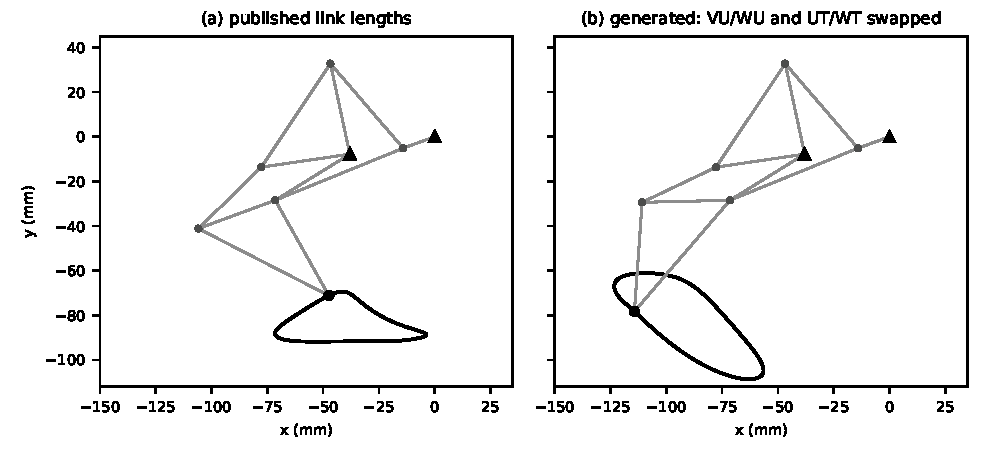
\includegraphics[width=0.82\textwidth]{figures/jansen.pdf}
\caption{Jansen leg solved from (a) the published link lengths and (b) the \texttt{SIM.params} of a simulator generated by the larger model, which swapped \texttt{VU}/\texttt{WU} and \texttt{UT}/\texttt{WT}. Grey: linkage at one crank angle; black curve: path of the foot T over one crank revolution; triangles: fixed pivots. Both pages run and animate without errors.}\label{fig:jansen}
\end{figure}

All 20 failures were confirmed by hand. They fall into four classes:
\begin{itemize}
\item \emph{Misremembered design knowledge} (15). In all nine faulty Jansen legs the generator recalled the published numbers but assigned some of them to the wrong links, or scrambled them, for example a crank of 38 instead of 15. Figure~\ref{fig:jansen} shows a leg with two swapped pairs: the page runs, animates and looks like a Strandbeest, but the foot no longer has a flat ground-contact segment. With the lengths of the first two faulty legs, the flat part of the foot path shrank from 36\% to 6\% of the cycle and the stride from 49 to 11~mm. All five lambda linkages from the smaller model used ordinary four-bar proportions instead of Chebyshev's, and the larger model once placed the tracing point at the middle of the coupler instead of its extended end. A direct check of path straightness agrees with the proportion check on all ten lambda simulators: the four that pass trace a near-straight segment (1\% of the crank length) over $200^\circ$, and the six that fail have no such segment. No correct alternative design was rejected.
\item \emph{Violated assembly conditions} (4). Two planetary sets had $Z_s+Z_r=100$, not divisible by three, so three equally spaced planets cannot mesh with both sun and ring. Two Watt six-bars had a second loop that cannot close for part of the cycle.
\item \emph{Runtime failure} (1). A four-bar threw an exception on load because it assigned to a read-only property.
\item \emph{Geometry outside the contract} (1, not in the table). In one Geneva drive the cut-out of the locking disc faced away from the pin, so the wheel is not locked during dwell and the disc overlaps the wheel during indexing. The oracle cannot see this, because it checks markers, not the outline of the drawn parts; the VLM reviewer found it (Section~\ref{sec:rq2}).
\end{itemize}
Mechanisms whose design rule is a relation that the description implies produced no errors at all. This holds for the cam (0/10), whose motion law the description states, and for the Peaucellier--Lipkin linkage (0/10), whose conditions the models stated correctly in every case. The difference between models is clearest on the lambda linkage: 5/5 wrong for the smaller model versus 1/5 for the larger ($p=0.048$).

\paragraph{Another vendor} The two DeepSeek models of phase~8 show the same pattern on the two design-knowledge mechanisms. One of the 20 replies was cut off at the output limit and contained no page, so 19 simulators ran. The larger model was wrong on 9 of 10 (Jansen 5/5, lambda 4/5) and the smaller on 5 of 9 (Jansen 4/4, lambda 1/5). Every failure was a DESIGN failure of the proportion check, and inspection confirmed each one. As with Claude, the Jansen legs used the published numbers but assigned some of them to the wrong links. None of the five faulty lambda linkages had Chebyshev's proportions. Here the relation between models is reversed: the larger DeepSeek model erred more often on lambda than the smaller. Error rates on recalled design knowledge are therefore high across vendors, but which model is worse is not stable.

\subsection{RQ2: what the oracle and the VLM detect}\label{sec:rq2}

\paragraph{Seeded mutants} The oracle detected all 24 detailed-specification mutants, all 15 spec-lite mutants, and, with the drift check, the gamed mutant. On the 24 detailed-specification mutants, checks that need no ground truth (META and structural checks) already caught 17: all state, length and phase faults, three of four branch faults and two of four direction faults. The remaining seven, a four-bar on the crossed branch, two reversed directions and four panel faults, need the kinematic solution. The VLM reviewer detected 20 of 24 mutants when the numeric panel was visible and 14 of 24 without it. Its detection of 10--15\% length errors fell from 4/4 to 1/4. From its explanations, the VLM recovered lengths mainly by reading the panel and solving the kinematics itself, not by inspecting the drawing. Paired by mutant, the oracle's advantage is significant against the VLM without panel (10 versus 0 discordant mutants, exact McNemar $p=0.002$) but not against the VLM with panel (4 versus 0, $p=0.125$). Among the four mutants the VLM missed with the panel visible, it saw a $12$--$20^\circ$ slot offset of the Geneva wheel but attributed it to perspective.

\paragraph{Natural errors} On the 15 renderable simulators of phase~2, the VLM found 5 of the 6 oracle-detected errors and reported 1 false positive on 9 correct simulators. It missed the planetary assembly violation, which is invisible in a rendering, but found the Geneva disc error that the oracle cannot see. On the 44 new simulators of phase~5 it had 7 true positives, 1 false negative (again a planetary tooth-count violation) and 4 false positives, all Geneva drives. The marker data show these wheels index by exactly $72^\circ$ per driver turn; the reviewer misread intermittent motion as a fault. The VLM was also unstable: a fresh review of the same unchanged files at the start of repetition~2 called three faulty simulators correct, among them the Geneva drive it had flagged before.

The two oracles are complementary. The executable oracle catches errors of design knowledge and invisible errors (assembly conditions, state, panel values) deterministically, in about 0.2~s and with no model calls. The VLM catches shape errors outside the marker contract but misses invisible ones, produces false alarms on intermittent motion, and costs about 52{,}000 tokens per review.

\subsection{RQ3: the oracle as an acceptance gate for repair}\label{sec:rq3}

In two preliminary phases, one round of repair fixed 3 of 7 faulty files whether the feedback came from the oracle (as check names and magnitudes), the VLM or nobody. With three rounds, specific oracle feedback fixed 6 of 6 against 4/6 (coarse oracle), 2/6 (VLM) and 0/6 (self-refine). Tables~\ref{tab:rounds} and~\ref{tab:repair} report the full design.

% generated by make_tables.mjs from pilot/iter5/*/summary.json -- do not edit by hand
\begin{table}[!htbp]
\caption{File-runs passing the oracle after each repair round, phases 5--6 pooled (22 file-runs; round 0 = generated file)}\label{tab:rounds}
\begin{tabular}{@{}lcccc@{}}
\toprule
Arm & r0 & r1 & r2 & r3 \\
\midrule
location + value & 0 & 16 & 22 & 22 \\
location only & 0 & 12 & 14 & 14 \\
check + magnitude & 0 & 8 & 10 & 10 \\
VLM review in the loop & 0 & 5 & 5 & 5 \\
Self-refine (no feedback) & 0 & 6 & 6 & 6 \\
\botrule
\end{tabular}
\end{table}

% generated by make_tables.mjs from pilot/stats/stats.json -- do not edit by hand
\begin{table*}[t]
\caption{Iterative repair (at most three rounds): file-runs whose simulator passes the oracle at the end, by feedback arm. Assembly/constraint errors: Watt six-bar, planetary, four-bar crash. Design knowledge: Jansen (phases 5--6) and Chebyshev lambda (phase 7). The VLM arm was not run for the lambda file-runs (n/a).}\label{tab:repair}
\begin{tabular}{@{}lcccc@{}}
\toprule
Feedback arm & Assembly / constraint & Design knowledge, Haiku & Design knowledge, Sonnet & All \\
\midrule
Oracle, location + value & 8/8 & 13/13 & 7/7 & 28/28 \\
Oracle, location only & 8/8 & 0/13 & 7/7 & 15/28 \\
Oracle, check + magnitude & 8/8 & 0/13 & 3/7 & 11/28 \\
VLM review in the loop & 5/8 & 0/8\textsuperscript{a} & 0/6\textsuperscript{a} & 5/22\textsuperscript{a} \\
Self-refine (no feedback) & 6/8 & 0/13 & 1/7 & 7/28 \\
\botrule
\end{tabular}
\footnotetext[a]{Lambda file-runs excluded (no VLM arm).}
\end{table*}


Over the 22 file-runs of phases 5--6, feedback with location and correct value fixed all 22, all within two rounds. It was followed by location only (14), check and magnitude (10), self-refinement (6) and VLM in the loop (5). The arms differ (Cochran's $Q=44.5$, $df=4$, $p=5\times10^{-9}$). After Holm correction, full oracle feedback beats every other arm (location only $p=0.047$, coarse $p=0.004$, VLM $p=1.5\times10^{-4}$, self-refine $p=2.7\times10^{-4}$), and location-only beats VLM ($p=0.027$) and self-refinement ($p=0.047$). Location-only versus coarse (4 versus 0 discordant file-runs) and coarse versus VLM or self-refinement are not significant. With each source file counted once (20 file-runs including lambda, four arms) the conclusions do not change: full feedback 20/20 versus location only 10/20 (Holm $p=0.008$), coarse 8/20 ($p=0.002$) and self-refinement 4/20 ($p=1.8\times10^{-4}$).

The difficulty splits by error class. Assembly and runtime errors were repaired with any oracle feedback (8/8 in all three oracle arms) and often even without (self-refinement 6/8, VLM 5/8); the arms do not differ significantly on this class ($Q$ test $p=0.064$). Design-knowledge errors were repaired almost only with oracle feedback, as RQ4 details.

The two loops without an executable gate failed in characteristic ways. VLM-driven loops stopped 12 times on a ``correct'' verdict while the oracle still failed the file, and the VLM never recognised the planetary tooth-count error, so its arm did worse than self-refinement even on assembly errors. Self-refinement stopped when the repairer answered \texttt{NO\_CHANGE}, and all 17 such answers on faulty Jansen legs declared the file correct; 10 of them stated explicitly that the link lengths ``match Jansen's holy numbers''. In one case the repairer stated that nothing was wrong with a four-bar that did not load.

\paragraph{Is a repairer needed at all?} Because the full report states the correct values, we also ran a deterministic baseline without any model. It takes the values that the location + value report on the original file gives as ``expected'' and writes them into the page. Two variants were tried:
\begin{itemize}
\item \emph{Patching \texttt{SIM.params} at load time}: 0 of 28 file-runs passed (20 source files). The design check then passed, but every page had built its link geometry from the old lengths, so the drawing no longer matched the parameters.
\item \emph{Rewriting the numeric literals in the page source}, the more favourable variant, so that the geometry is built from the corrected values: 11 of 28 file-runs passed (9 of 20 source files; Table~\ref{tab:repair}).
\end{itemize}
The patch cannot touch assembly, tooth-count or runtime errors, for which the report names a violated condition but no value (0/8). On design-knowledge errors it fixed 11 of 20. The other nine still failed for three reasons. With the corrected lengths, some pages solved the linkage on a different assembly branch. In others, parts no longer met at shared joints. In the rest, a frame marker or the tracing point was drawn by separate code that the patch did not reach. The model given the same report fixed all 28. The LLM is therefore not a transcriber of numbers. It keeps the code, the drawing and the panel consistent with the corrected design, and it repairs faults for which no value exists.

\subsection{RQ4: how specific must feedback be?}\label{sec:rq4}

Pooling the design-knowledge file-runs (Jansen, phases 5--6, and lambda, phase 7), the result depends strongly on the repairing model (Table~\ref{tab:repair}):
\begin{itemize}
\item The smaller model fixed 13 of 13 with location and value and 0 of 13 with location only, coarse feedback or no feedback (Cochran's $Q=39$, $p=1.7\times10^{-8}$; each pair with the full arm exact McNemar $p=2.4\times10^{-4}$, Holm $p=0.001$; counting each source file once, 10/10 versus 0/10, Holm $p=0.012$).
\item The larger model fixed 7 of 7 with location and value \emph{and} 7 of 7 with location only, 3 of 7 with coarse feedback and 1 of 7 without feedback.
\item With location only, the two models differ sharply (7/7 versus 0/13, Fisher $p=1.3\times10^{-5}$); with location and value they do not (7/7 versus 13/13, $p=1$).
\end{itemize}
The lambda linkage, added to test whether this pattern was specific to Jansen, reproduced it. The smaller model fixed 5/5 with values and 0/5 in each of the three other arms; the larger model's single faulty file was fixed in every arm, including self-refinement.

The repairers' replies show why location is not enough for the smaller model. The ``looks swapped with'' hints let it undo permutations. In two lambda files this left a single wrong link, the distance to the tracing point, which has to be recalled (five crank lengths). It never recovered that value in three rounds. Instead it substituted other proportions it believed to be classical (several different sets across files and rounds, none correct), back-computed a length from the reported error magnitude (four attempts, all wrong, since the minimax formula is not in the feedback), or answered \texttt{NO\_CHANGE}. On Jansen, 9 of the 40 location-only attempts were \texttt{NO\_CHANGE} replies claiming that the lengths matched the published numbers and that the checker's mapping must be wrong. The larger model, given only the names of the wrong links, supplied the published values from memory. With coarse feedback, it twice inferred the wrong Jansen link from the error magnitude itself, the only route by which coarse feedback fixed a Jansen leg.

\subsection{Reliability of the oracle}\label{sec:reliability}
The reference simulators pass, and every seeded mutant is detected. Every oracle failure on a generated simulator was confirmed by hand, so we observed no false positives. The single false negative is the Geneva disc of Section~\ref{sec:rq1}, which lies outside the contract. To exclude passes obtained by moving markers instead of parts, we audited all passing generated simulators and all passing final repaired versions, 146 files, for marker drift: all had a drift of zero. One repairer explicitly tried this tactic, saying it had set markers ``directly from the solved points'', but its version still failed the design check. After we added the drift check and changed the Jansen scale estimate, we regraded all 661 earlier verdicts. 660 were unchanged, and the gamed mutant moved from pass to fail. Rule violations by agents were rare. One of 155 phase-5 repair attempts ran a Python command despite the instruction, and one phase-7 attempt stopped without writing a reply, asking instead to be told the classical proportions.
